\documentclass[compress]{beamer}
\usepackage{graphicx,amsmath,amsthm,verbatim,bm}
\usepackage{longtable}
%\usetheme{Copenhagen}
%\useoutertheme[{options}]{tree}
%\setbeamertemplate{footline}[page number]
%\useoutertheme{infolines}
%\setbeamertem plate{headlirne}{}
\useinnertheme{circles}
\usepackage{comment}
\setbeamertemplate{footline}[frame number]
%\usepackage{times}
%\usepackage[tbtags]{amsmath}
%\usepackage{amssymb}
\usepackage{amsfonts}
\usepackage{multirow}
%\usepackage{slfortheorems}
\usepackage{epsfig}
\usepackage{graphicx}
\usepackage[small]{caption}
\usepackage[square]{natbib}
%\newcommand{\newblock}{}
\bibpunct{(}{)}{;}{a}{}{,}
\bibliographystyle{ims}
%\usepackage[letterpaper]{geometry}
\usepackage{color}
\setlength{\parindent}{0pt}
\usepackage{bbding}
\usepackage{longtable, booktabs}
\usepackage{amsfonts}
\usepackage{lipsum}
\usepackage{tikz} 
\usetikzlibrary{arrows, snakes, backgrounds, patterns, matrix, shapes, fit, 
calc, shadows, plotmarks}
\useinnertheme{circles}
\usepackage{tabularx}

\newcommand{\clusters}{\bm{\kappa}}
\newcommand{\cluster}[1]{\kappa_{#1}}
\newcommand{\sizes}{\bm{\mu}}
\newcommand{\size}[1]{\mu_{#1}}

\newcommand{\edist}{\bm{\gamma}}
\newcommand{\shape}{\eta}
\newcommand{\rate}{s}
\newcommand{\betaA}{u}
\newcommand{\betaB}{v}



\usepackage{tkz-berge}
\usetikzlibrary{fit,shapes}

\usepackage{calc}
\usetikzlibrary{decorations.markings}

\tikzstyle{vertex}=[circle, draw, inner sep=0pt, minimum size=6pt]
\newcommand{\vertex}{\node[vertex]}
\newcounter{Angle}


\usepackage{tabularx}

\let\oldvec\vec
\let\oldcomment\comment
\renewcommand{\comment}[1]{\textcolor{blue}{[#1]}}
\renewcommand\vec{\bm}
\newcommand{\simfn}{\texttt{sim}} % similarity function
\newcommand{\truncsimfn}{\underline{\simfn}} % truncated similarity function
\newcommand{\partfn}{\texttt{PartFn}} % partition function
\newcommand{\distfn}{\texttt{dist}} % distance function
\newcommand{\valset}{\mathcal{V}} % attribute value set
\newcommand{\entset}{\mathcal{E}} % set of records that make up an entity
\newcommand{\partset}{\mathcal{P}} % set of entities that make up a partition
\newcommand{\1}[1]{\mathbb{I}\!\left[#1\right]} % indicator function
\newcommand{\euler}{\mathrm{e}} % Euler's constant
\newcommand{\eber}{\texttt{EBER}} % Name of Bayesian ER model
\newcommand{\secref}[1]{\S\ref{#1}} % Section reference



\usepackage{listings}
\usepackage[ruled,lined]{algorithm2e}
\def\algorithmautorefname{Algorithm}
\SetKwIF{If}{ElseIf}{Else}{if}{then}{else if}{else}{endif}

\usepackage{longtable}



\theoremstyle{plain}
\usepackage{amsfonts}
\usepackage{epsfig}
\usepackage{graphicx}
%\usepackage[small]{caption}

\usepackage{zref-savepos}

\newcounter{restofframe}
\newsavebox{\restofframebox}
\newlength{\mylowermargin}
\setlength{\mylowermargin}{2pt}

\newenvironment{restofframe}{%
    \par%\centering
    \stepcounter{restofframe}%
    \zsavepos{restofframe-\arabic{restofframe}-begin}%
    \begin{lrbox}{\restofframebox}%
}{%
    \end{lrbox}%
    \setkeys{Gin}{keepaspectratio}%
    \raisebox{\dimexpr-\height+\ht\strutbox\relax}[0pt][0pt]{%
    \resizebox*{!}{\dimexpr\zposy{restofframe-\arabic{restofframe}-begin}sp-\zposy{restofframe-\arabic{restofframe}-end}sp-\mylowermargin\relax}%
        {\usebox{\restofframebox}}%
    }%
    \vskip0pt plus 1filll\relax
    \mbox{\zsavepos{restofframe-\arabic{restofframe}-end}}%
    \par
}


\usepackage{tikz}
\usetikzlibrary{arrows}

%\usepackage[usenames,dvipsnames]{xcolor}
\usepackage{tkz-berge}
\usetikzlibrary{fit,shapes}

\usepackage{calc}
\usetikzlibrary{decorations.markings}

%\tikzstyle{vertex}=[circle, draw, inner sep=0pt, minimum size=6pt]
%\newcommand{\vertex}{\node[vertex]}
%\newcounter{Angle}



%%%to add in new counter for slides in beamer
\newcommand{\beginbackup}{
   \newcounter{framenumbervorappendix}
   \setcounter{framenumbervorappendix}{\value{framenumber}}
}
\newcommand{\backupend}{
   \addtocounter{framenumbervorappendix}{-\value{framenumber}}
   \addtocounter{framenumber}{\value{framenumbervorappendix}} 
}


\newcommand*\oldmacro{}
\let\oldmacro\insertshortauthor
\renewcommand*\insertshortauthor{
  \leftskip=.3cm
\insertframenumber\,/\,\inserttotalframenumber\hfill\oldmacro}




\excludecomment{notbeamer}
\includecomment{beamer}

\newcommand{\lam}{\mathbf{\Lambda}}	
\newcommand{\bX}{\mathbf{X}}
\newcommand{\bY}{\mathbf{Y}}

\title[Data Cleaning Pipeline]
{Data Cleaning Pipeline}
\author[Rebecca C. Steorts, beka@stat.duke.edu]{Rebecca C. Steorts} 



%\begin{figure}[htbp]
%\begin{center}
%\includegraphics{pics/banner}
%%\caption{default}
%\label{default}
%\end{center}
%\end{figure}

%\date{August 13, 2019}




\begin{document}
\begin{frame}
\titlepage
\end{frame}


\frame{
\frametitle{Objectives}

\begin{itemize}
\item Cover some basic pipeline approaches from the database literature. 
\item Understanding how they integrate with one another.
\item Understand pros and cons about the approaches. 
\item These methods are a basic starting point for moving forward with more complex methods. 
\item Due to their simplicity, they are used in many production or industrial pipelines. Let's try and understand why that would be the case by the end of the lecture. 
\end{itemize}




}


\frame{
\frametitle{Goals} 

\begin{enumerate}
\item Enumerating a census. 
\item Enumerating those that have died in a conflict (such as Syria).
\item Predicting those in poverty in small regions from survey data. 
\item Predicting results of elections from voter registration data. 
\item Predicting housing/rental prices from Zillow data. 
\end{enumerate}

\vspace*{1em}

Each task may contain duplicated information, which is problematic for the underlying task at hand. 

}

\frame{
%\frametitle{Motivation} 

\begin{figure}[htbp]
\begin{center}
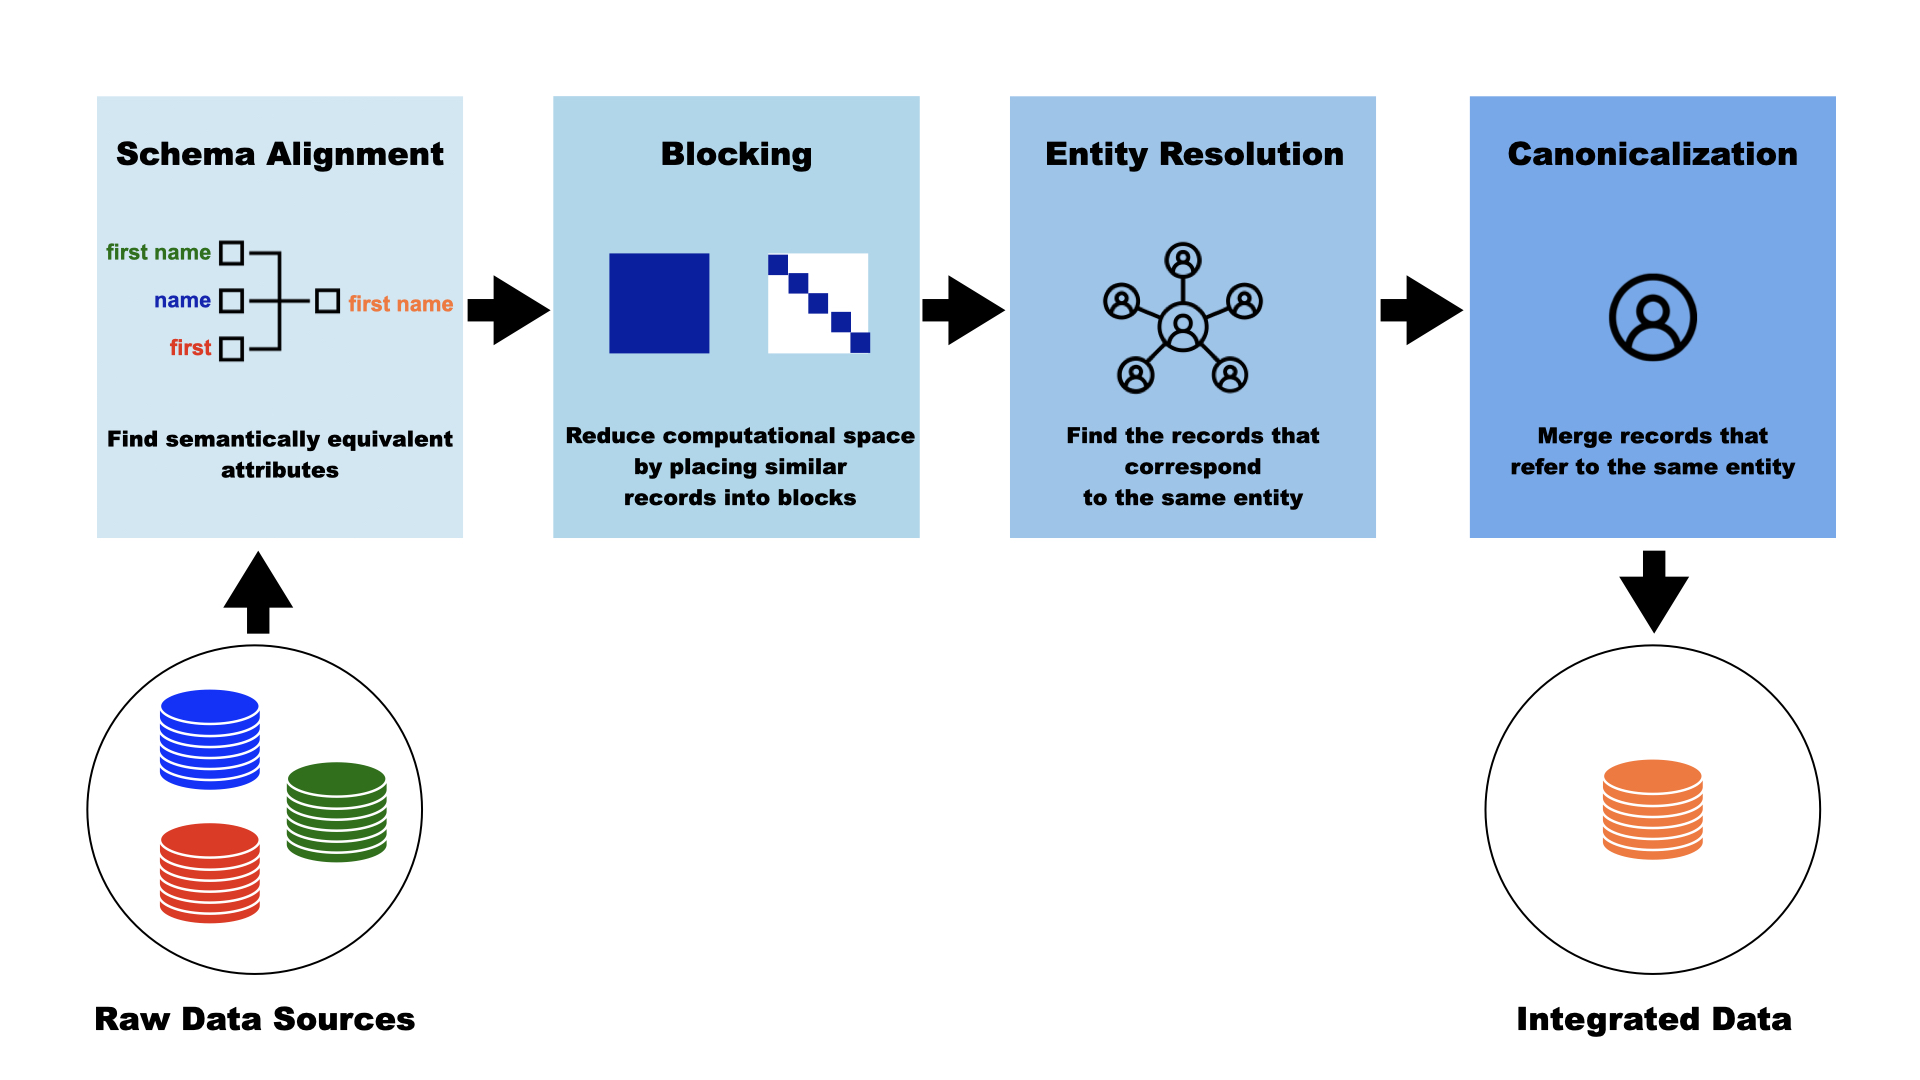
\includegraphics[width=\textwidth]{data-pipeline-picture.001}
%\caption{default}
\label{default}
\end{center}
\end{figure}

}

\frame{

\begin{enumerate}
\item The most important information in the pipeline is known as the profile or the record. 
\vspace*{1em}

\item Each profile or record is a collection of attributes/fields about a person, organization, or object. 

\vspace*{1em}

\item Commonly collected attributes about people are name, address, phone number, gender, among other types of information.

\end{enumerate}
}


\frame{
%\frametitle{Motivation} 

\begin{figure}[htbp]
\begin{center}
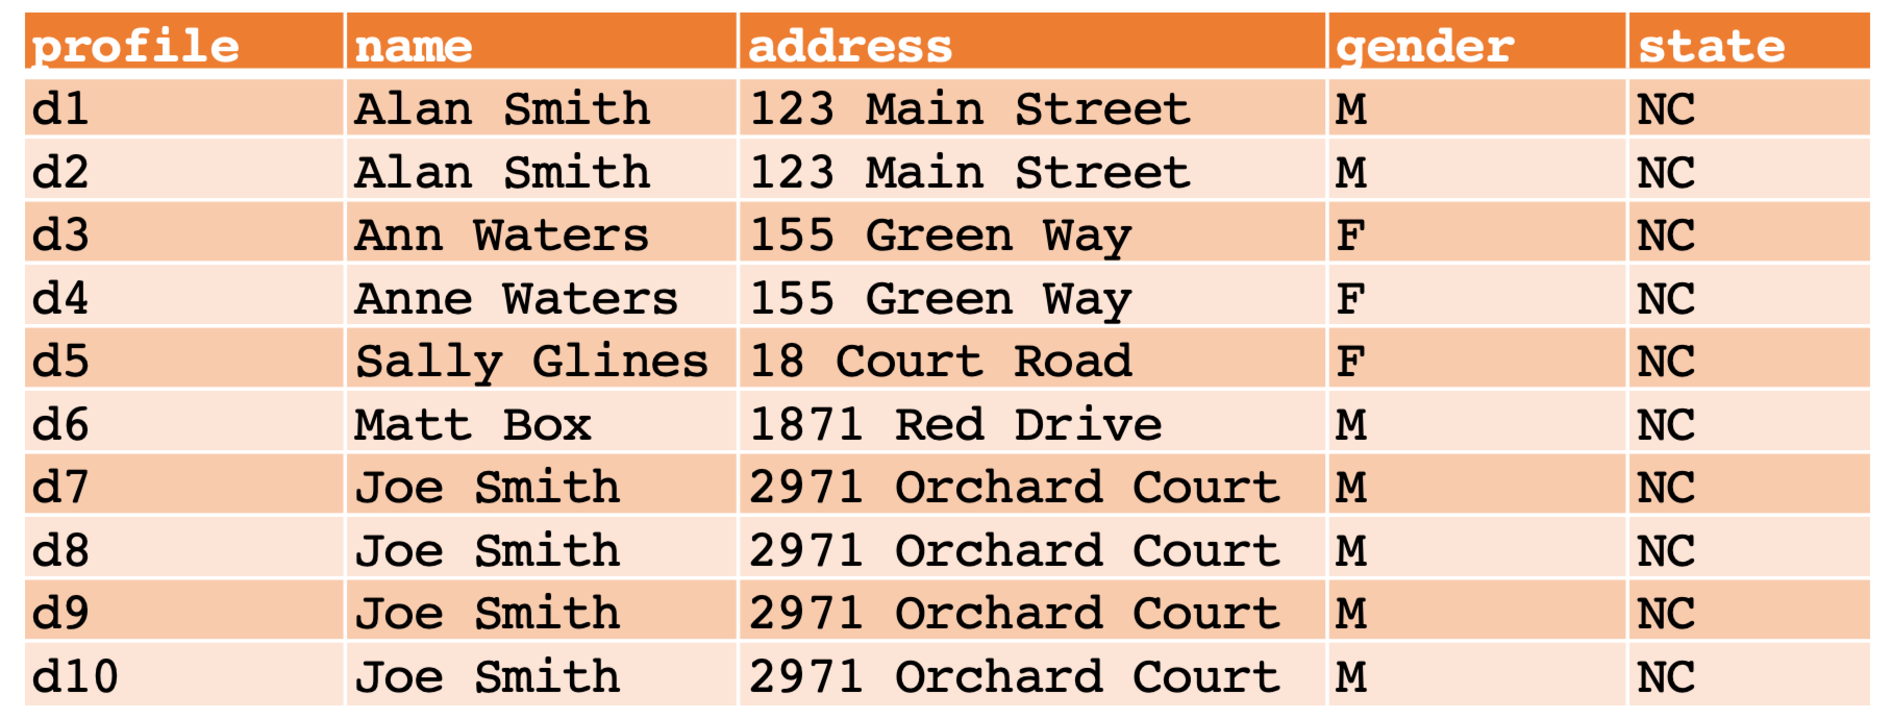
\includegraphics[width=\textwidth]{database1}
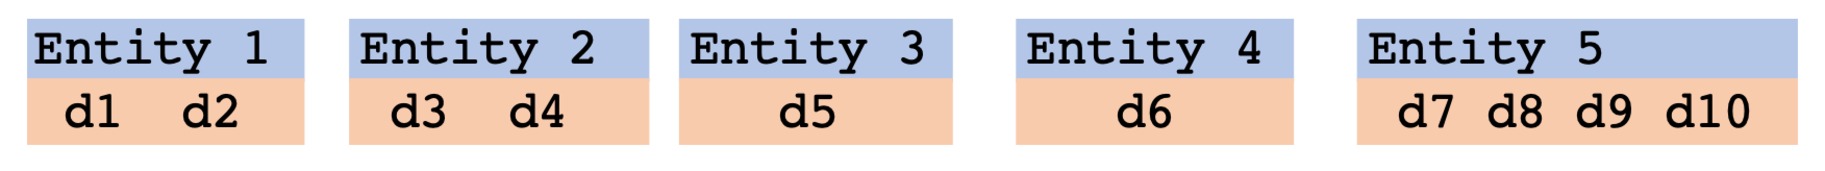
\includegraphics[width=\textwidth]{database1-entities}
%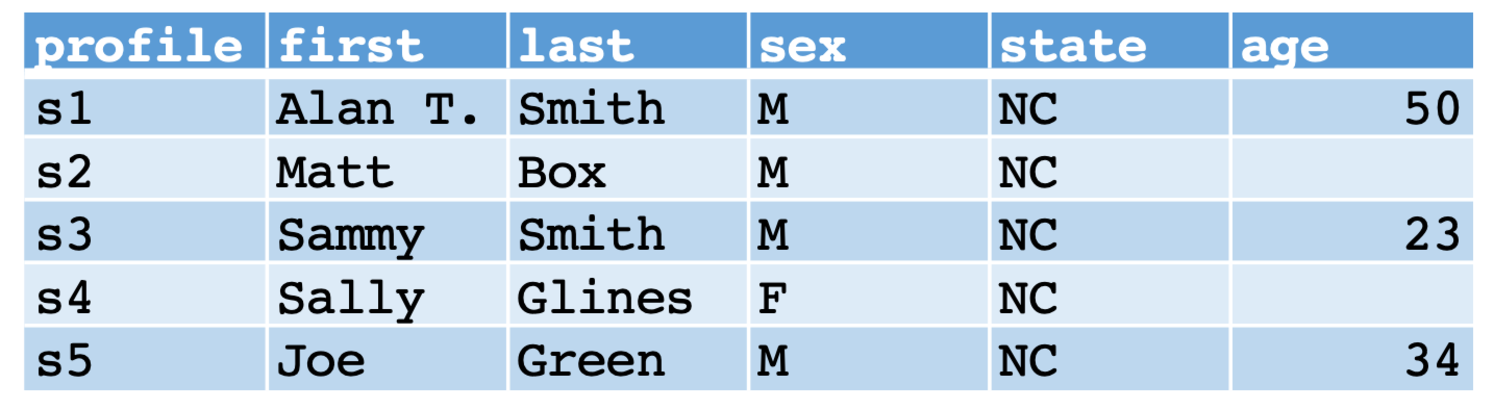
\includegraphics[width=0.6\textwidth]{database2}
%\caption{An example of noisy, structured data source:  the input data source (DS) and 
% the corresponding true entities. }
\label{default}
\end{center}
\end{figure}

%Let $e_i$ denote entity $i.$ 
%
%$e_1 = \{D1, D2\}, e_2 = \{D3, D4\}, e_3 = \{D5\}, e_4 = \{D6\}, e_5 = \{D7, D8, D9, D10\}.$

}

\frame{
%\frametitle{Motivation} 

\begin{figure}[htbp]
\begin{center}
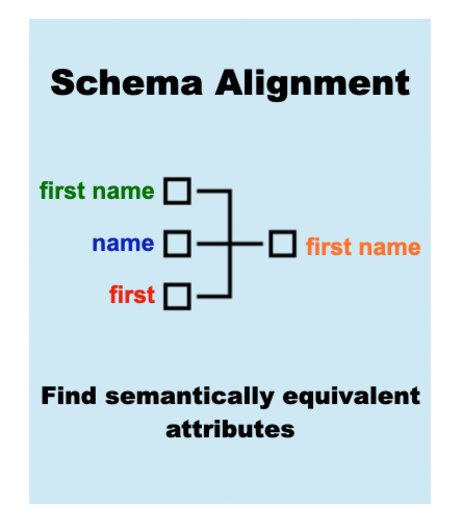
\includegraphics[width=0.5\textwidth]{schema}
%\caption{An example of noisy, structured data source: (a) the input data source (DS) and 
%(b) the corresponding true entities. Citation: Papadakis et. al (2021).
%}
\label{default}
\end{center}
\end{figure}

}

\frame{

\begin{enumerate}
\item It is important that we align attributes when our schemata are disparate. 
\item The goal is to create alignments of attributes based upon the following:
\begin{enumerate}
\item Similarity 
\item Structure
\item Attributes Present
\end{enumerate}
\end{enumerate}
\vspace*{1em}

Formally, this is known as identifying ``semantically equivalent attributes'', such as first name, first, and name. 
\vspace*{1em}

[Bernstein et al., 2011, Madhavan et al., 2001]. 

}

\frame{

\begin{enumerate}
\item This stage leverages the attribute values from the records/profiles. 
\item Schema knowledge is used (if available). 
\item The goal is to learn attribute mappings between the data sources.
\item The goal is to also find ``transformations, correspondences, or rules between the attributes."  [Tejada et al., 2002, Yan et al., 2001]. 
\item Common transformations are used, such as: ``Dr." to ``Drive" or ``3rd" to ``third" [Active Atlas, Tejada et al., 2002].
\end{enumerate}

}


\frame{
%\frametitle{Motivation} 

\begin{figure}[htbp]
\begin{center}
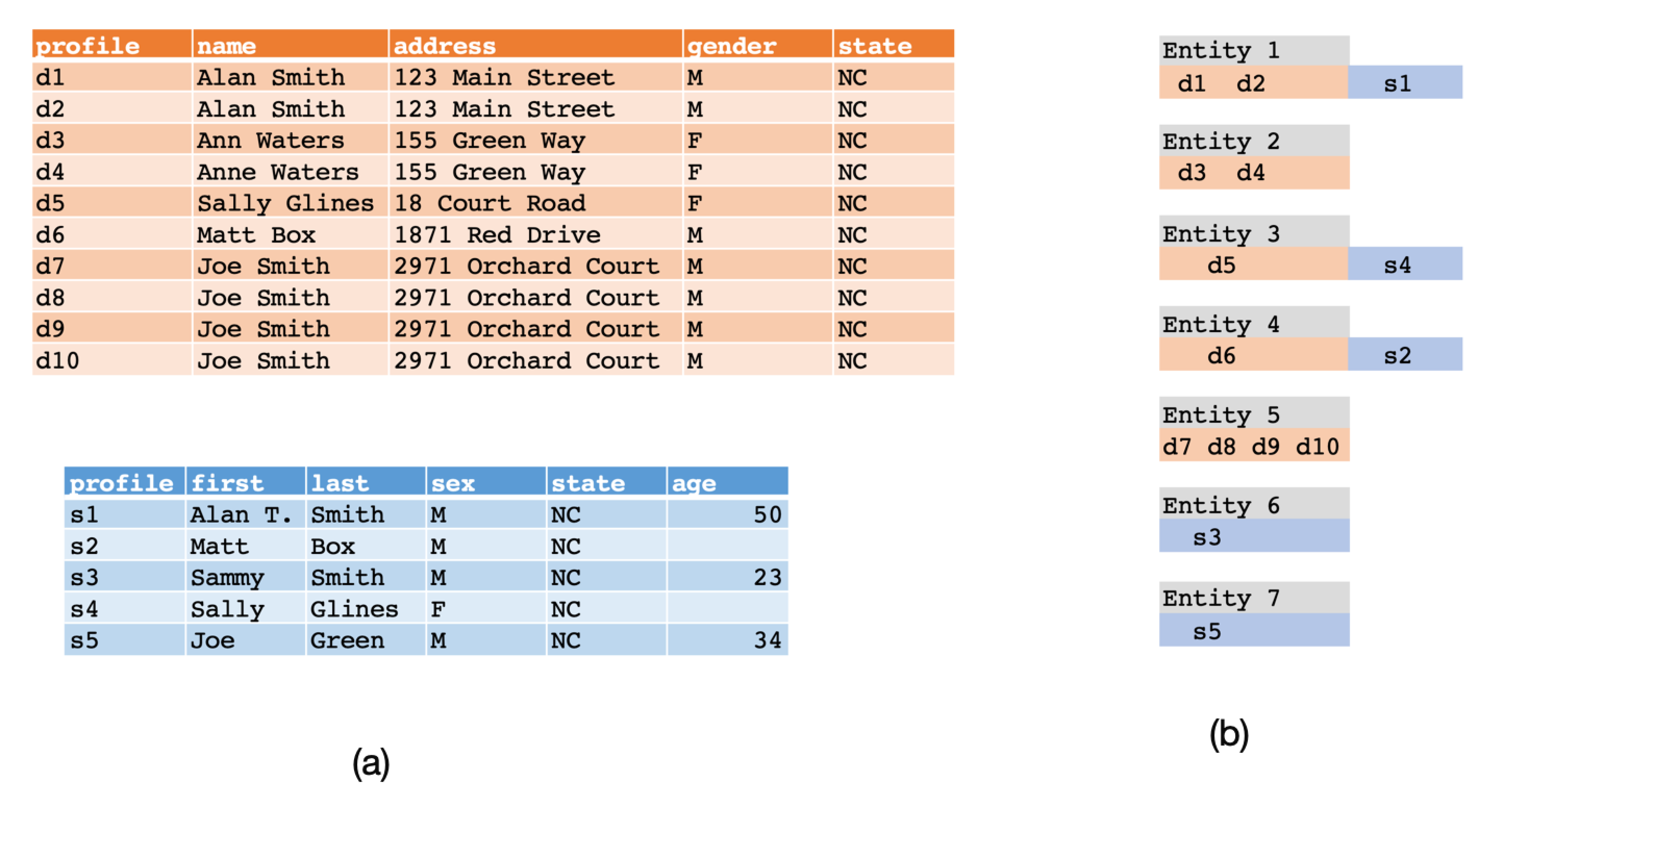
\includegraphics[width=\textwidth]{databases-two}
%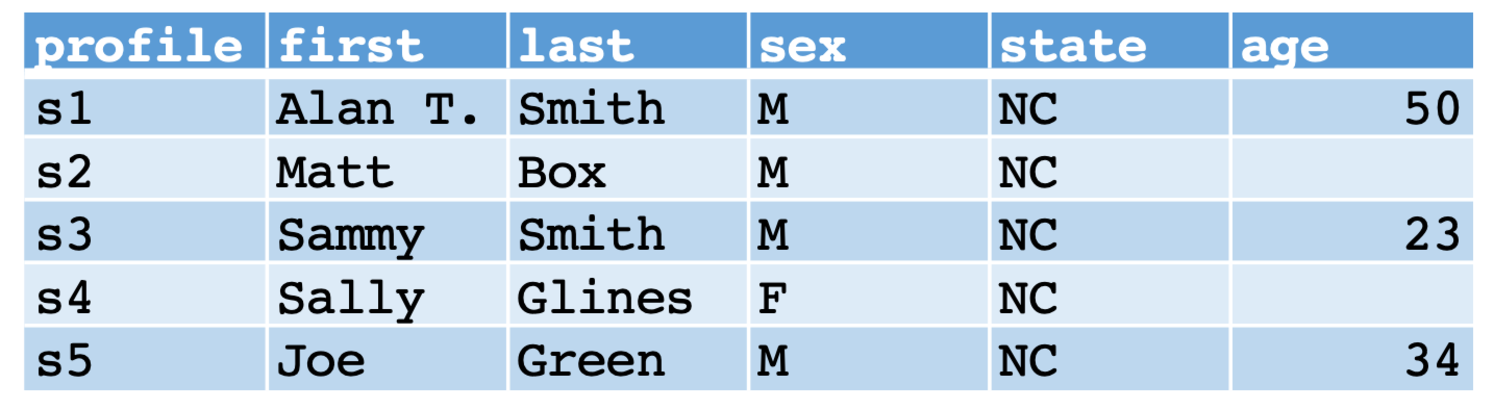
\includegraphics[width=0.5\textwidth]{database2}
%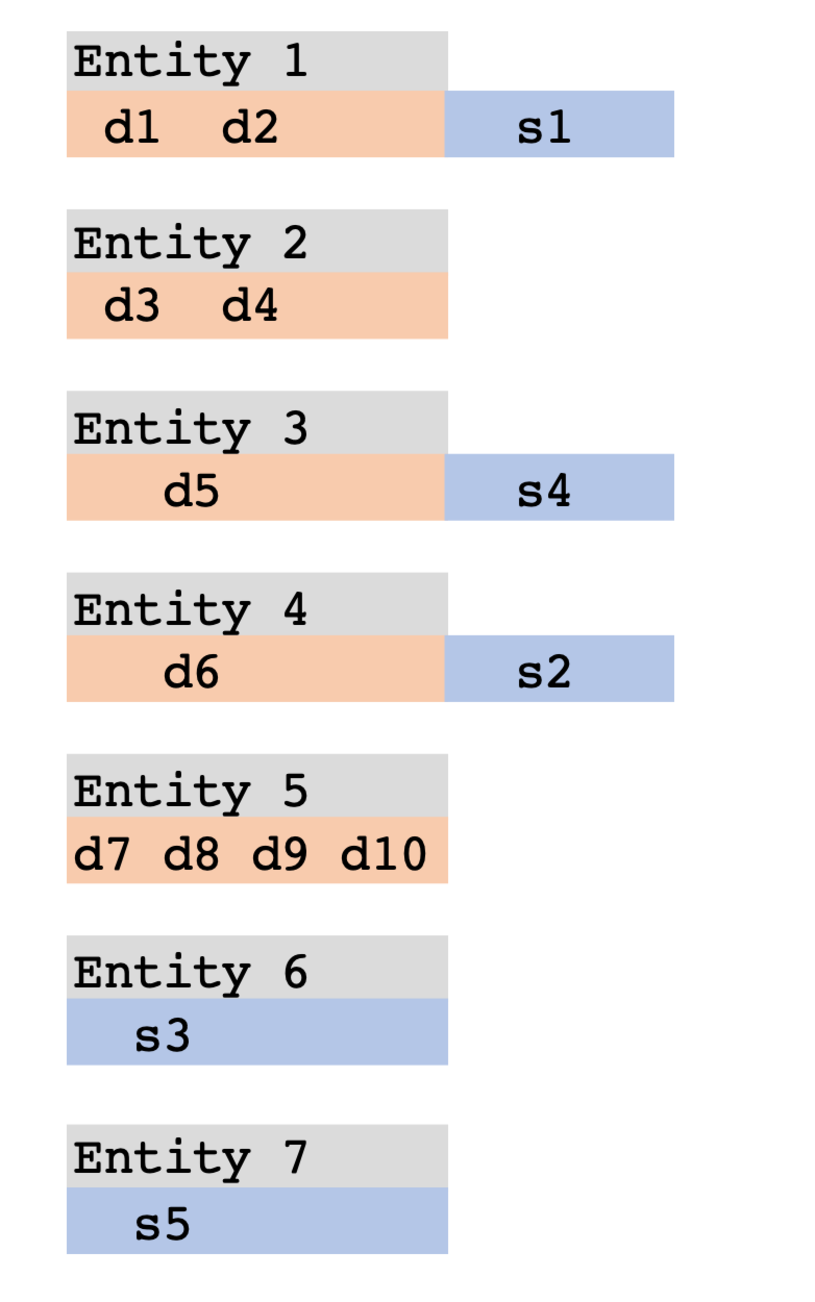
\includegraphics[width=0.5\textwidth]{database2-entities}
\caption{An example two databases: (a) the input databases and 
(b) the corresponding entities. 
}
\label{default}
\end{center}
\end{figure}

}

\frame{
%\frametitle{Motivation} 

\begin{figure}[htbp]
\begin{center}
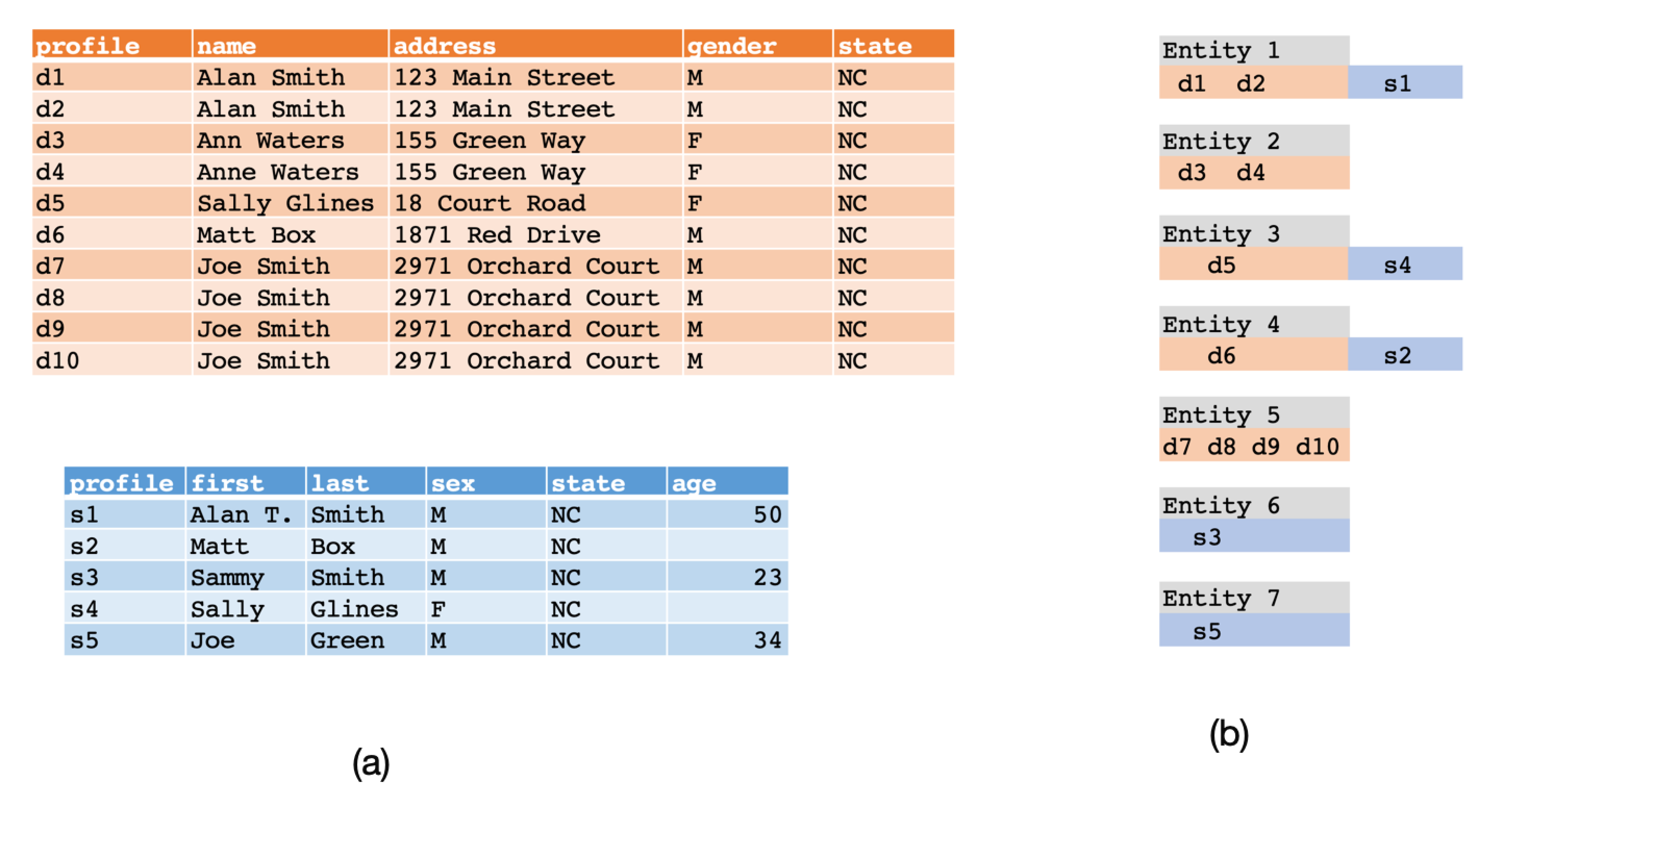
\includegraphics[width=\textwidth]{databases-two}
%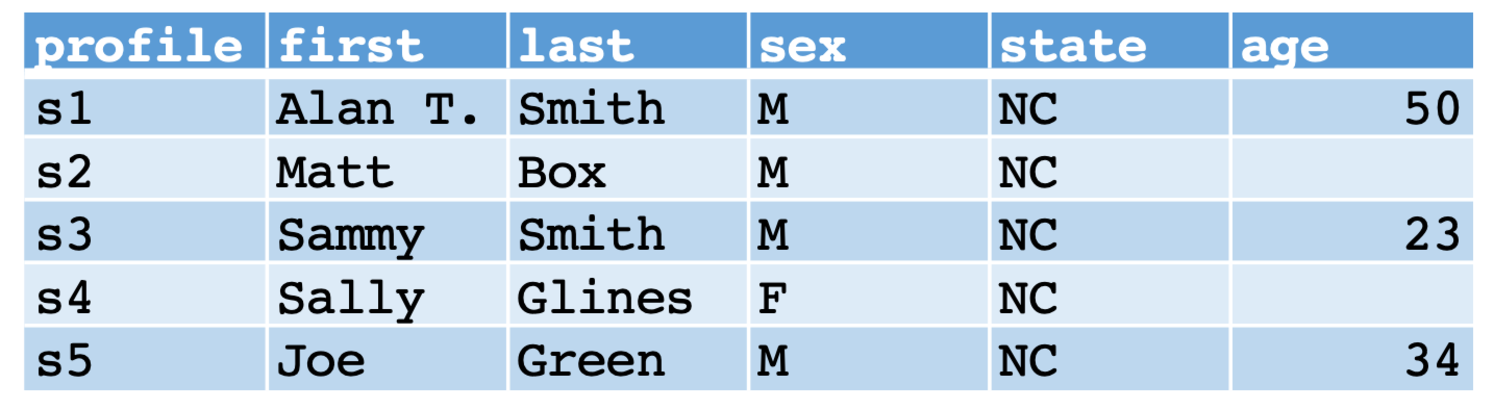
\includegraphics[width=0.5\textwidth]{database2}
%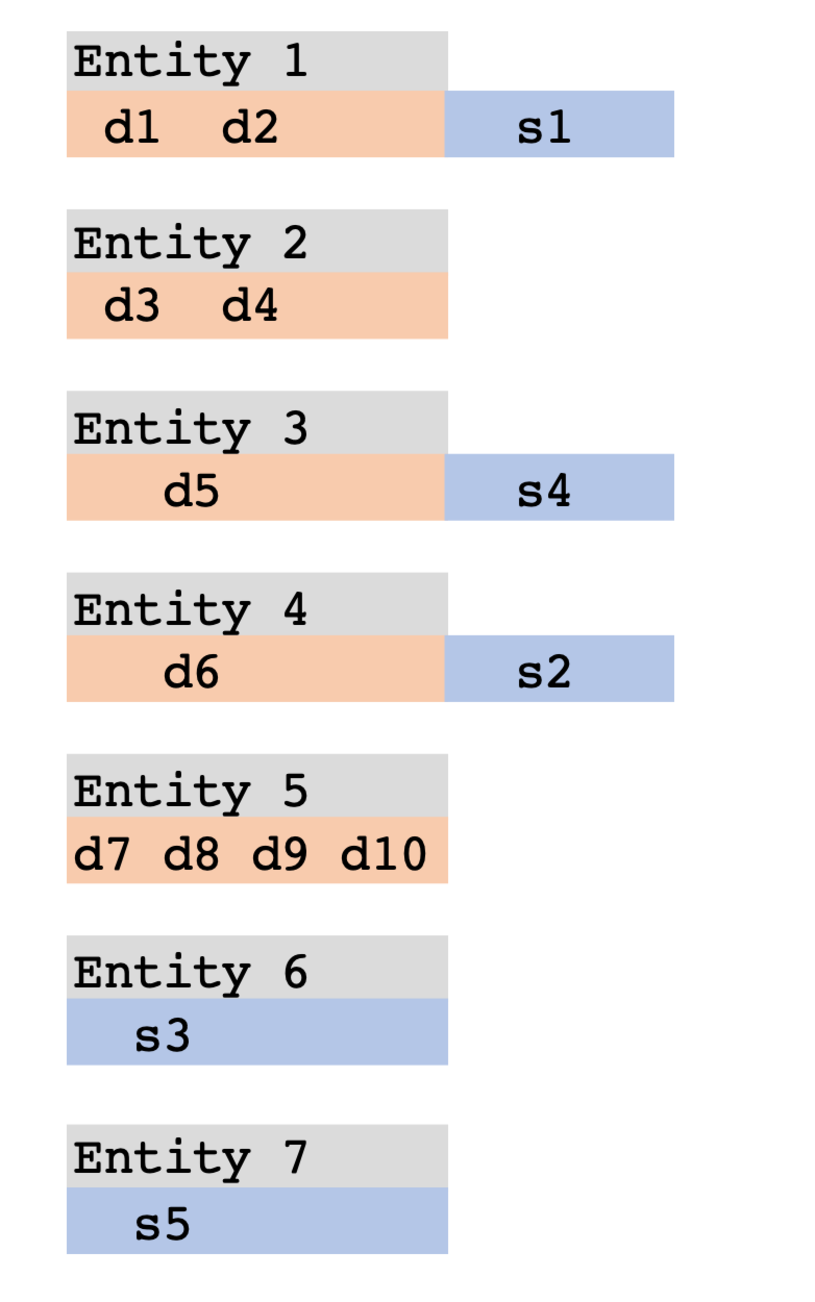
\includegraphics[width=0.5\textwidth]{database2-entities}
\caption{An example two databases: (a) the input databases and 
(b) the corresponding entities. 
}
\label{default}
\end{center}
\end{figure}

Alignment rules: first and last/name; sex and gender.

}



\frame{

\begin{enumerate}
\item It is important that the schema are coded for all databases in the same way.
\item The naming structured should be well organized and documented in a relational database. 
\item More information can be found in Papadakis et. al (2021) for more information and other illustrations.
\end{enumerate}

}

\frame{
%\frametitle{Motivation} 

\begin{figure}[htbp]
\begin{center}
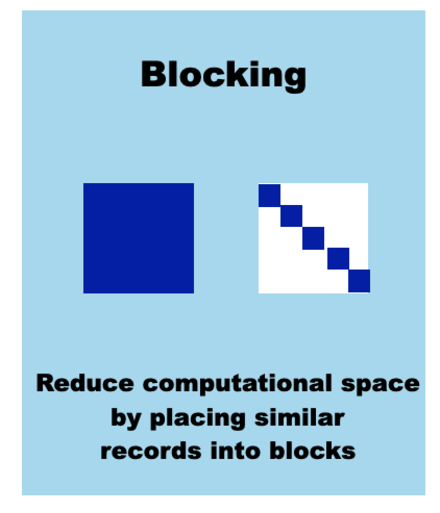
\includegraphics[width=0.5\textwidth]{blocking}
%\caption{An example of noisy, structured data source: (a) the input data source (DS) and 
%(b) the corresponding true entities. Citation: Papadakis et. al (2021).
%}
\label{default}
\end{center}
\end{figure}

}

\frame{

\begin{enumerate}
\item Blocking operates in a schema-aware fashion, assuming that the input data adheres to a known schema or to aligned schemata. 
\item Based on this assumption and respective domain knowledge, the most suitable attributes are used for extracting one or more representative signatures from each profile. 
\item These signatures are called blocking keys and are composed of (combinations of) parts of values from the most informative attributes. 
\item Assuming that these keys reflect the overall similarity of profile pairs, profiles with identical or similar keys are placed into the same block to be compared 
in the entity resolution stage.
\end{enumerate}


}


\frame{

\begin{enumerate}
\item Standard Blocking (SB) [Fellegi and Sunter, 1969] requires an expert to manually define a part or a transformation of one or more attribute values as the single blocking key of each profile. 
\item Every profile is then placed in the block corresponding to its blocking key. 
\item To increase its robustness, a multi-pass functionality is applied in practice, i.e., SB is combined with several different definitions of blocking keys.
\end{enumerate}


}

\frame{

\begin{enumerate}
\item One common type of blocking is using q-grams (or shingling) [Christen, 2012b, Papadakis et al., 2015].
\item This converts SB keys into sub-sequences of q characters (q-grams) and defines a block for every distinct q-gram.
\end{enumerate}

There are multiple extensions to these in the computer science and database management literature.

}

\frame{


\begin{enumerate}
\item A record can be thought of as a string of characters.
\item A q-gram (or shingle) is a substring (or word) of length $q$ found within the record. 
\item We are interested in a set of k-grams that appear one or more times in the record.
\end{enumerate}

}

\frame{

Observe that in the manner of this approach, one finds the standard blocking (SB) key and then proceeds with another blocking approach or pass. 

\vspace*{1em}

In summary, the blocking stage is made into many blocking passes, iteratively. 

}



\frame{

How might we define a blocking criteria for these data sources?

}

\frame{

Define the blocking key the concatenation of the following three pieces of information: 
\begin{enumerate}
\item  (i) \{“Name,” Last2Characters\}, 
\item (ii) \{“Address,” Last2Characters\}, 
\item and (iii) \{“Gender,” FirstCharacter\}.
\end{enumerate}

}

\frame{
%\frametitle{Motivation} 

\begin{figure}[htbp]
\begin{center}
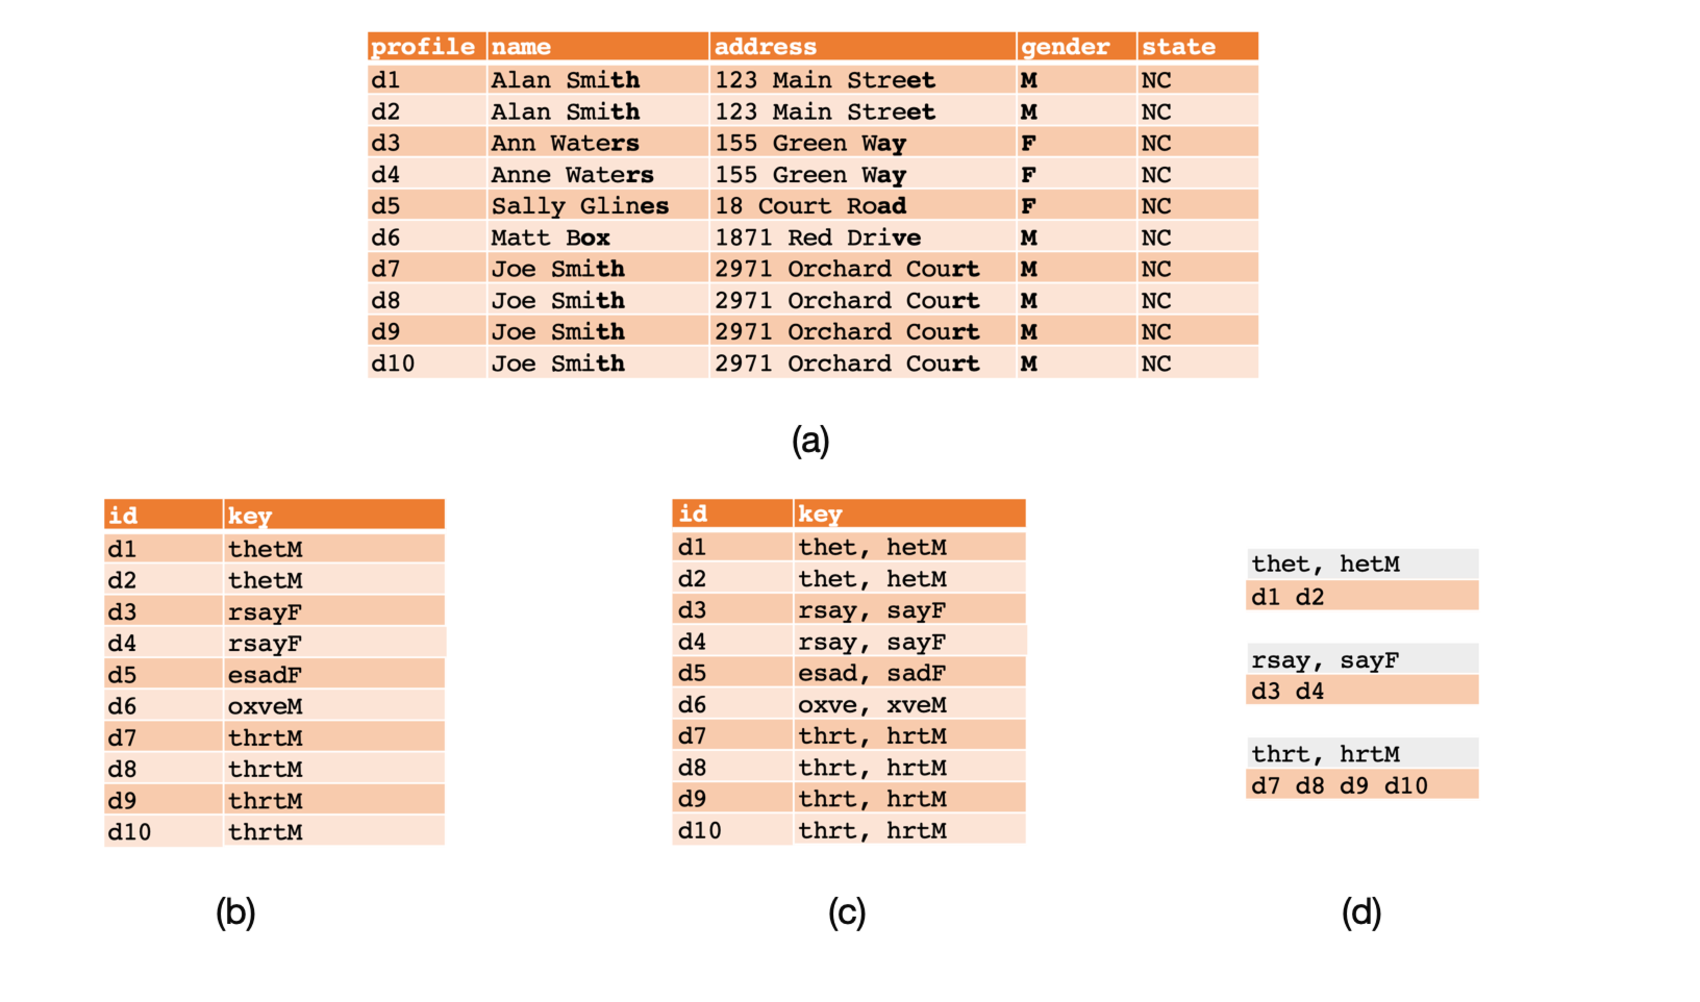
\includegraphics[width=\textwidth]{blocking-criteria}
\caption{
(a) the input data source with bolded information used in blocking keys, (b) the blocking keys via SB, (c) the blocking keys of 4-grams blocking, and (d) the blocks of 4-grams blocking.
}
\label{default}
\end{center}
\end{figure}



}

\frame{


\begin{figure}[htbp]
\begin{center}
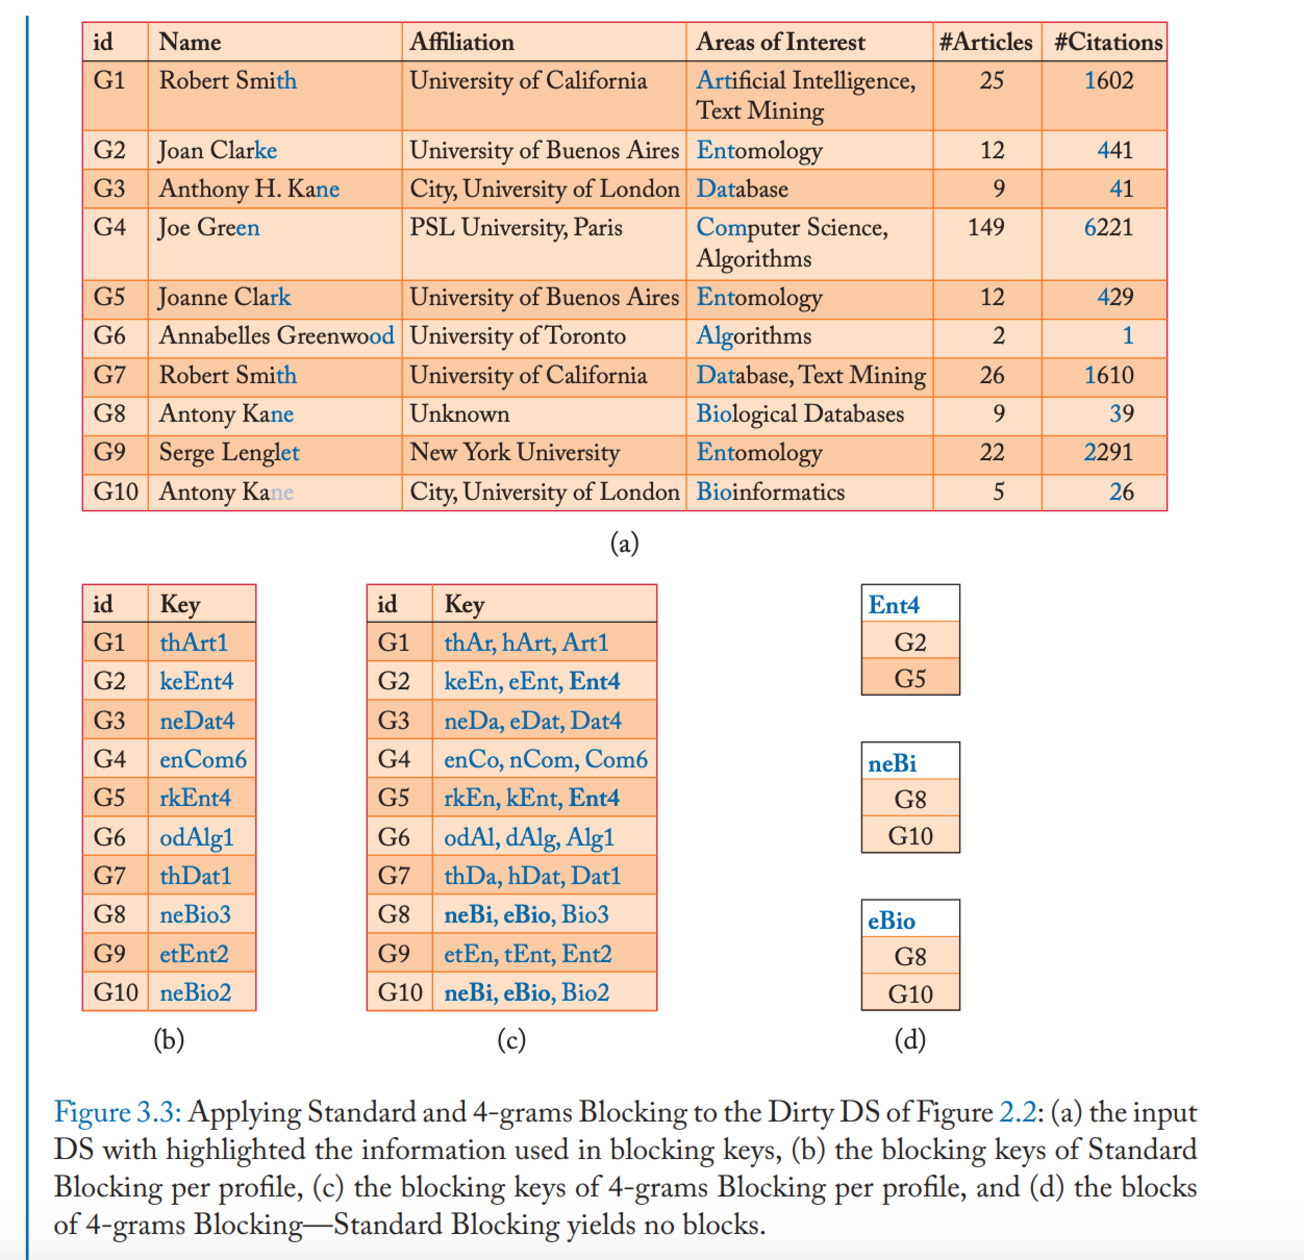
\includegraphics[width=0.75\textwidth]{blocking-book}
\caption{
Blocking from Pap. et. al (2022), page 20. Observe that no blocks result from the full pass. 
}
\label{default}
\end{center}
\end{figure}


}


%\frame{
%
%Define the blocking key the concatenation of the following three pieces of information: 
%\begin{enumerate}
%\item  (i) \{“Name,” Last2Characters\}, 
%\item (ii) \{“Areas of Interest,” First3Characters\}, 
%\item and (iii) \{“Citations,” FirstCharacter\}.
%\end{enumerate}
%
%}

%\frame{
%%\frametitle{Motivation} 
%
%\begin{figure}[htbp]
%\begin{center}
%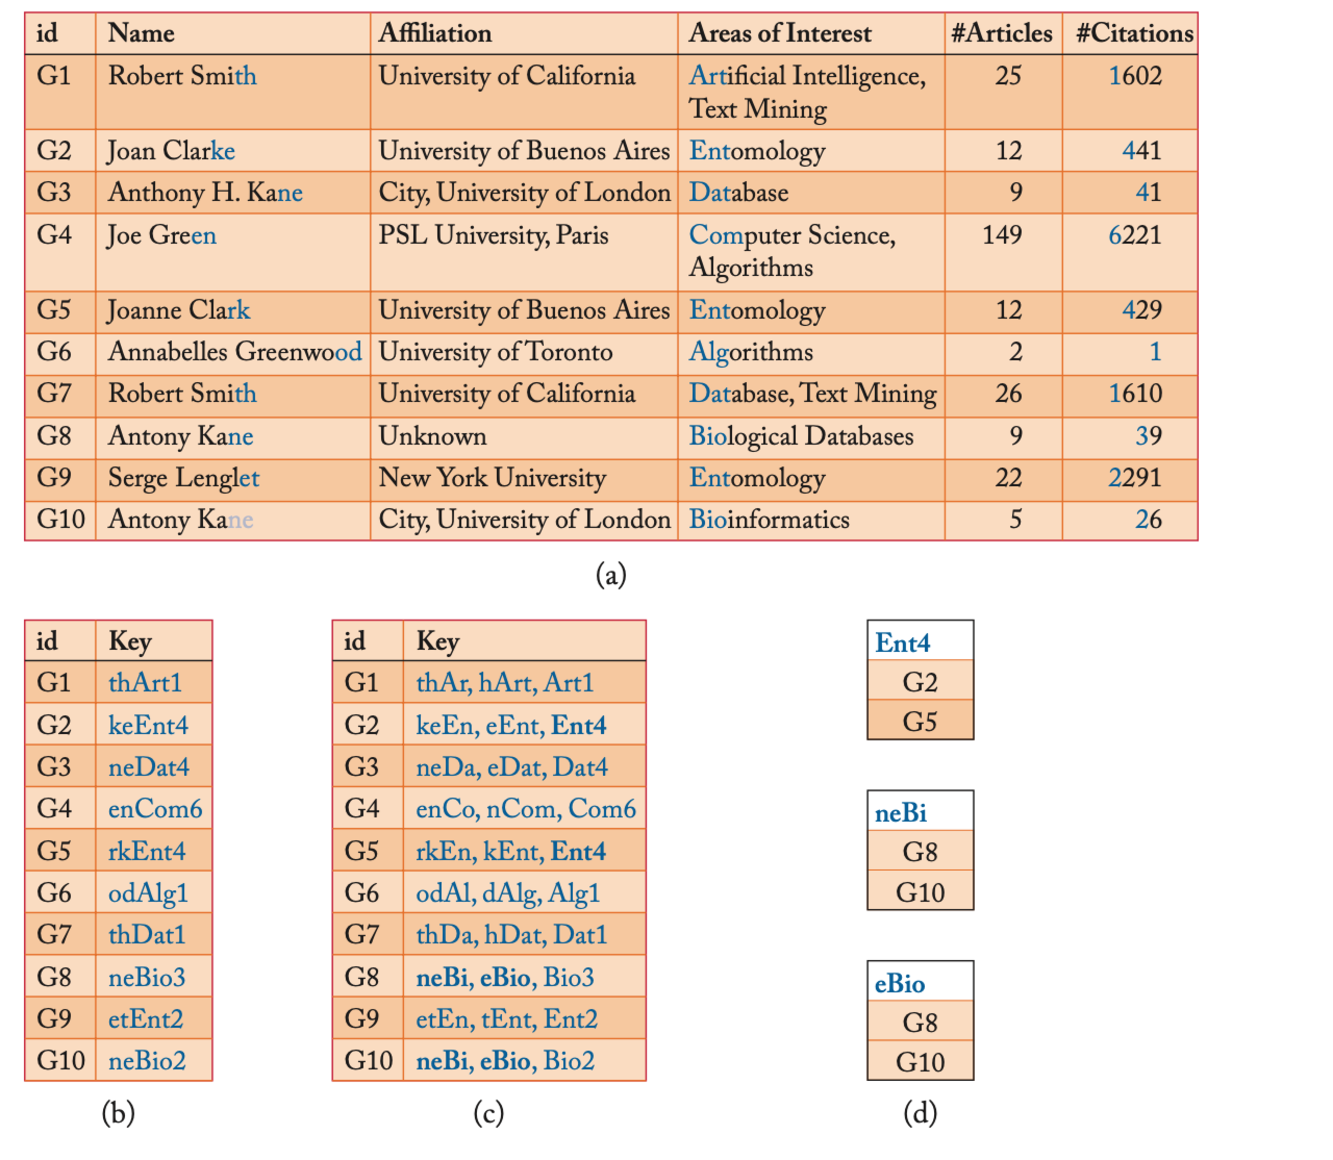
\includegraphics[width=0.8\textwidth]{figure3-3}
%\caption{
%(a) the input DS with highlighted the information used in blocking keys, (b) the blocking keys via SB, (c) the blocking keys of 4-grams Blocking, and (d) the blocks of 4-grams Blocking.
%}
%\label{default}
%\end{center}
%\end{figure}
%
%}

\frame{

There are many other ways that blocking criteria can be defined and many options are reviewed in Papadakis et. al (2021).

\vspace*{1em}

We have just gone through an iterative approach that is simple to code up. What might be limitations of this approach in practice?

}

\frame{
%\frametitle{Motivation} 

\begin{figure}[htbp]
\begin{center}
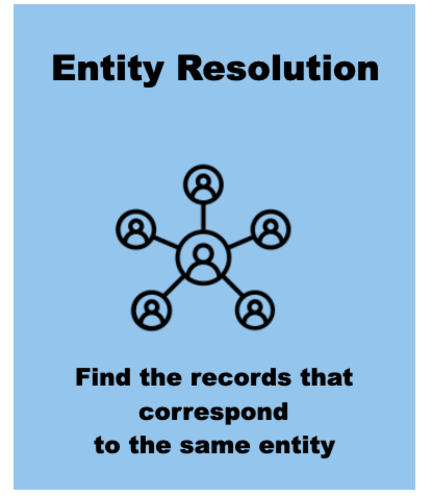
\includegraphics[width=0.5\textwidth]{entity-resolution}
%\caption{An example of noisy, structured data source: (a) the input data source (DS) and 
%(b) the corresponding true entities. Citation: Papadakis et. al (2021).
%}
\label{default}
\end{center}
\end{figure}

}

\frame{
%\frametitle{Motivation} 

\begin{figure}[htbp]
\begin{center}
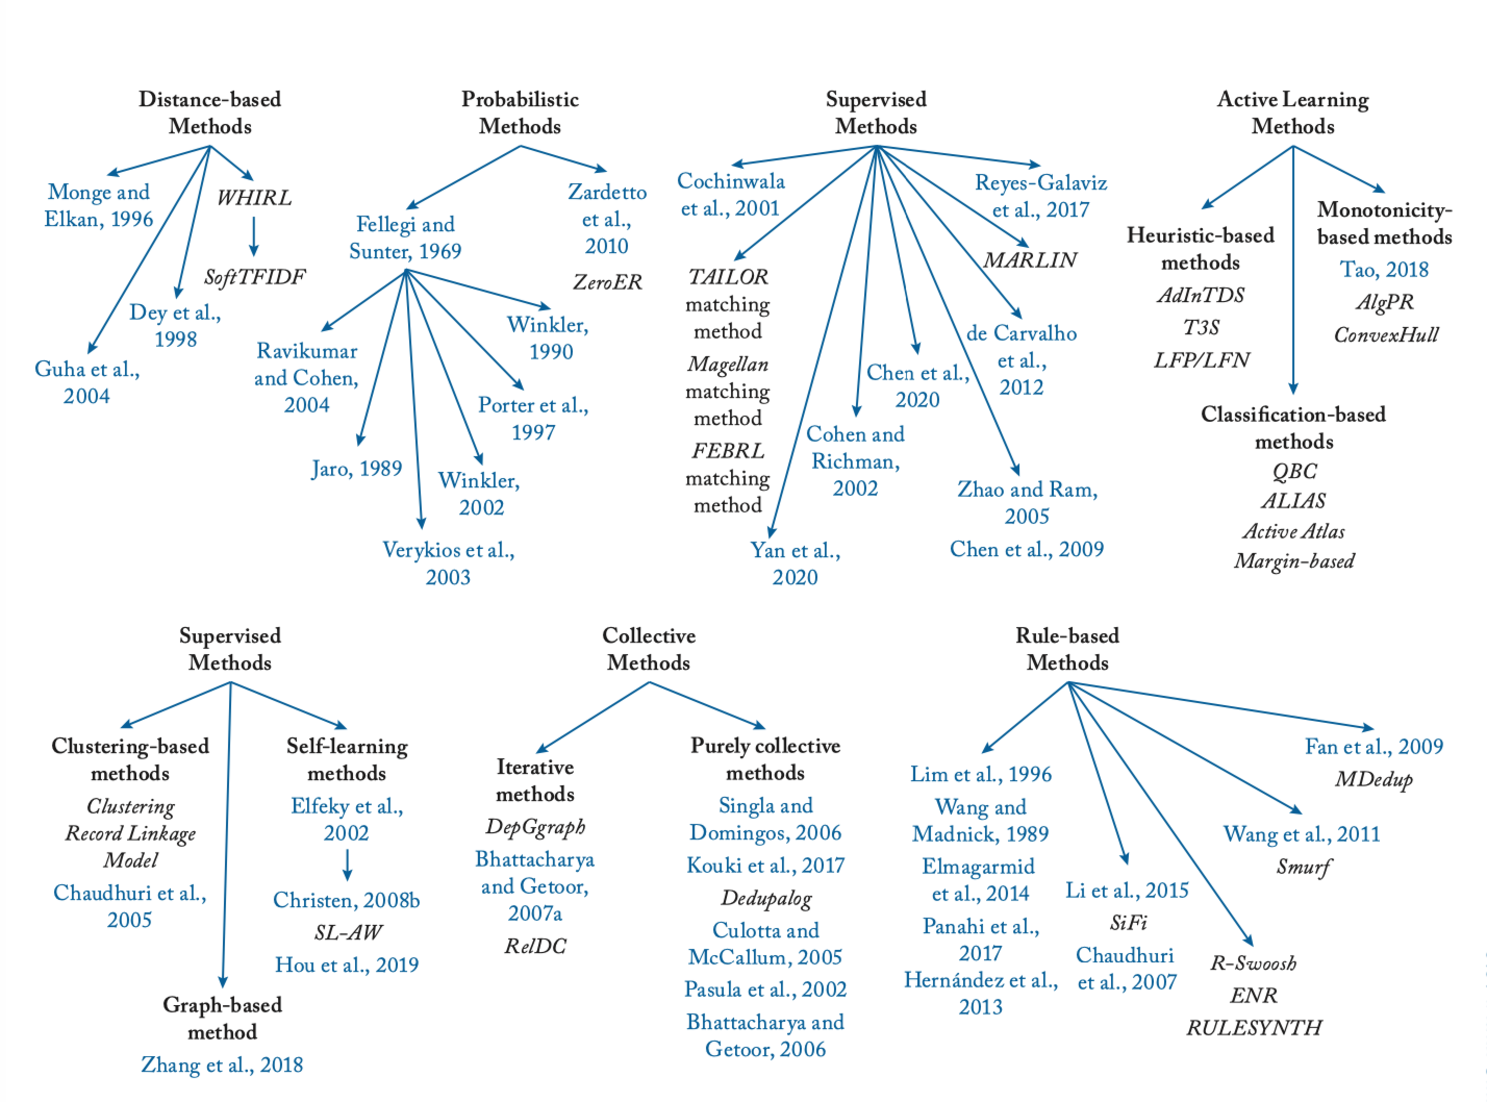
\includegraphics[width=\textwidth]{er-methods}
\caption{Citation: Papadakis et. al (2021).
}
\label{default}
\end{center}
\end{figure}

}


\frame{
%\frametitle{Motivation} 

\begin{figure}[htbp]
\begin{center}
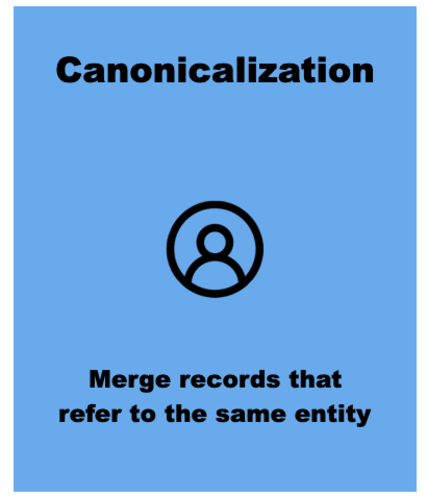
\includegraphics[width=0.5\textwidth]{canonical}
%\caption{An example of noisy, structured data source: (a) the input data source (DS) and 
%(b) the corresponding true entities. Citation: Papadakis et. al (2021).
%}
\label{default}
\end{center}
\end{figure}

}

\frame{

In summary, after all the stages the output is an integrated data set with unique identifiers that can be used in statistical analyses.


}

%\frame{
%
%\begin{enumerate}
%\item How can we work together to enable that these systems work well?
%\item How should these system be implemented? (scala, java, queries that work with scala/java)
%\item Should we avoid scripting languages such as python or R? 
%\item How do we get students/collaborators involved in the building of complex pipelines described? 
%\item Are there limiting resources at play?
%\end{enumerate}
%
%
%}

\frame{
\center
Thank you! \\
Questions?\\
Contact: beka@stat.duke.edu\\
\vspace*{1em}
\url{https://github.com/resteorts/record-linkage-tutorial}

\vspace*{1em}
\url{https://www.science.org/doi/10.1126/sciadv.abi8021}

\vspace*{1em}
\url{https://github.com/cleanzr}

\vspace*{1em}
Thank you to Anup Mathur, Krista Park, Kristen Olsen, and Jenny Thompson for conversations or feedback that led to this presentation. 

}


\end{document}